\documentclass[11 pt]{article}
\usepackage[utf8]{inputenc}
\usepackage[spanish, es-tabla]{babel}
\usepackage{graphicx}
\usepackage{multirow}
\usepackage{amsfonts}
\usepackage{anysize}
\marginsize{2.5cm}{2.5cm}{2.5cm}{2.5cm}
\parindent 1 cm
\usepackage{hyperref}
\hypersetup{
	colorlinks=true,
	linkcolor=black,
	urlcolor=cyan,
	citecolor=blue,
		}
\title{Situación actual de la Hepatitis E}
\author{Silvia Díaz Arco}
\date{14 de Diciembre de 2020}
\begin{document}
\maketitle
	\begin{abstract}
		Enlace al repositorio: \url{https://github.com/silviad95/Proyecto_final.git}\\\\
		La hepatitis viral es la forma más común de hepatitis. Entre los diferentes tipos posibles, la hepatitis E está emergiendo globalmente, siendo responsable de la mayoría de los casos de hepatitis aguda. El virus de la hepatitis E (VHE) es un virus de genoma ARN de cadena sencilla y polaridad positiva que pertenece al género {\em Orthohepevirus} de la familia {\em Hepeviridae}. Existen diversos genotipos, de los cuales el 1 y el 2 son patógenos humanos estrictos que se transmiten por la ruta fecal-oral debido a aguas contaminadas. Por ese motivo, son predominantes en los países en vías de desarrollo. Por otro lado, los genotipos 3 y 4 son de transmisión zoonótica, presentando una mayor variedad de huéspedes además del humano, siendo el reservorio principal el cerdo. Estos genotipos han adquirido interés al ser comunes en zonas industrializadas. La infección por VHE suele ser asintomática y autolimitante, pero precisamente por eso, en el mundo desarrollado se han dado casos de transmisión parenteral por donantes sanguíneos. Asimismo, se han documentado casos de hepatitis crónica en pacientes inmunocomprometidos. Para el diagnóstico de la infección, además de tener en cuenta el historial clínico del paciente, se recomienda la combinación de pruebas moleculares y serológicas. El tratamiento se basa en un antiviral no específico, ribavirina, no existiendo apenas terapias alternativas. Para la prevención del virus, solo existe una vacuna licenciada en China (Hecolin®), de la que no se ha probado su eficacia hacia el genotipo 3 ni su seguridad ante personas de riesgo.\\\\ 
		{\bf Palabras clave:} Hepatitis, viral, VHE, infección, genotipo	
	\end{abstract}
\newpage
\tableofcontents
\newpage
\section{Introducción}
\subsection{Hablemos de Hepatitis}
El término hepatitis significa “inflamación del hígado”. Es una afección global bastante frecuente que puede remitir espontáneamente, pero, que, en algunos casos, lleva al daño y destrucción de hepatocitos. Se pueden diferenciar entre hepatitis aguda (a corto plazo) y crónica (cuando la infección se prolonga a largo plazo). Las infecciones crónicas, sobre todo cuando se diagnostican tarde y no hay tratamiento, pueden generar daño permanente en el hígado pasando por la fibrosis (cicatrices), sangrado gastrointestinal, cirrosis (cicatrices permanentes), fallo en el hígado fulminante y/o un carcinoma hepatocelular que puede llevar al paciente a la muerte \cite{Mehta2020}.\\\\
Aunque la hepatitis se deba principalmente a infecciones virales, de las que hablaremos en el siguiente párrafo, también puede darse por causas no infecciosas. Así, la inflamación del hígado puede originarse por una enfermedad autoinmune \cite{Liberal2013}, por hígado graso \cite{NeuschwanderTetri2017} o por consumo excesivo de alcohol (hepatitis alcohólica) \cite{Chayanupatkul2014} y/o medicamentos \cite{Alempijevic2017}.\\\\
Existen 5 tipos principales de hepatitis virales, que se nombran de la A a la E. Aparte, se ha descrito la existencia de la hepatitis G. Normalmente se manifiesta como una coinfección con hepatitis B y C, aunque se desconoce su importancia en humanos. Otros virus, que generalmente no afectan principalmente al hígado, pero pueden causar hepatitis, son los citomegalovirus (CMV), el virus de Epstein-Barr (EBV) o el virus del herpes simple \cite{Mehta2020}. Las características que definen a cada tipo de hepatitis se muestra en la Tabla \ref*{tablahepatitis}.
\begin{table}[h!]
\begin{tabular}[c]{|c|c|c|c|c|c|c|}
	\hline
    	& {\bf VHA} & {\bf VHB} & {\bf VHC} & {\bf VHD} & {\bf VHE} \\
	\hline
	{\bf Género} & {\em Hepatovirus} & {\em Orthohepadnavirus}&{\em Hepacivirus}&{\em Virusoide}&{\em Orthohepevirus} \\
	\hline
	{\bf Genoma} & ARNss+ & ARNds parcial & ARNss+ & ARN & ARNss+\\
	\hline
	\parbox[c]{2 cm}{{\bf Fuente principal de transmisión}}
 & Ruta fecal-oral & \parbox[c]{2 cm}{Vertical, parenteral, sexual} & \parbox[c]{2 cm}{Contacto sanguíneo} & \parbox[c]{2 cm}{Coinfección o superinfección con VHB, contacto por sangre} & \parbox[c]{2 cm}{Ruta fecal-oral (países en desarrollo) Zoonótica (países desarrollados)}\\
	\hline 
	\parbox[c]{1.75 cm}{{\bf Tipo de infección}} & Aguda & Aguda y crónica & Crónica & \parbox[c]{2 cm}{Agrava pronóstico VHB} & Aguda y crónica\\
	\hline
	{\bf Tratamiento} & No específico & Sí (crónico) & Sí & Igual VHB & Sí (crónico)\\
	\hline
	{\bf Prevención} & Vacuna & Vacuna & Cribado & Igual VHB & \parbox[c]{2 cm}{Vacuna (solo en China)}\\
	\hline
\end{tabular}
\caption{Características de cada hepatitis. Significado de las siglas y referencias: VHA virus de la hepatitis A \cite{Thuener2017}, VHB virus de la hepatitis B \cite{You2014}, VHC virus de la hepatitis C \cite{Li2015}, VHD virus de la hepatitis D \cite{Rizzetto2015} y VHE virus de la hepatitis E \cite{Mohsen2017}.}
\label{tablahepatitis}
\end{table}

\subsection{Incidencia global}
En la figura \ref{laninigrafico} se muestra un gráfico circular que representa los datos de muertes por las diferentes hepatitis virales en 2017. Se puede observar que los pacientes mayores de 50 años son los que tienen más riesgo, ya que la tasa de mortalidad se dispara hacia 1.300.000. Asimismo, se puede ver que la principal causa de esas muertes es por la evolución crónica de la hepatitis B y C. En los individuos jóvenes, sin embargo, el fallo hepático agudo es el principal origen de esas muertes (89\%). Hay que destacar, además, que la hepatitis E fue causante de unos 1.500 fallecimientos en personas jóvenes y de unas 13.250 muertes en personas mayores de 50 años \cite{Lanini2019}.
\begin{figure} [h!] 
	\centering
	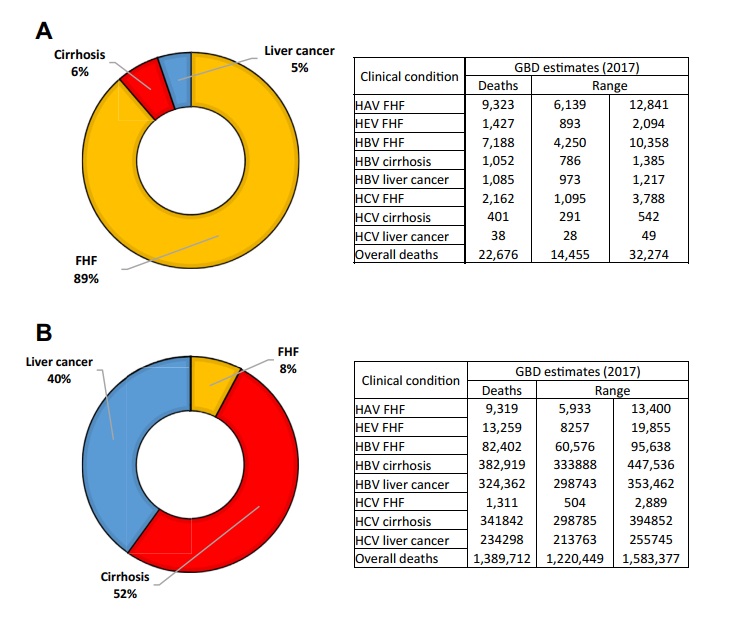
\includegraphics[width=0.75\linewidth]{imagenes/graficoincidenciahepatitis.png}
	\caption[loftitle]{Representación de muertes asociadas con las diferentes hepatitis virales en gente de menos de 50 años (A) y mayores de 50 años (B). Tomado de Lanini et al (2019) \cite{Lanini2019}}
	\label{laninigrafico}
\end{figure}

Actualmente, se reconoce el interés sanitario de la hepatitis E tanto en los países en desarrollo como en los países industrializados, donde se han dado casos de progresión de la hepatitis hacia una evolución crónica. Además, es una enfermedad emergente que es causante de la mayoría de casos de hepatitis aguda globalmente. Partiendo del creciente interés que ha suscitado esta infección, se ha querido realizar una búsqueda bibliográfica para recoger la información actualizada y completa que existe sobre esta patología. Con ello, también se pretende destacar dónde es necesario continuar investigando.

\section{Materiales y métodos}
\subsection{Tipo de estudio}
Para la comprobación del estado del arte se ha elegido, en primer lugar, llevar a cabo una revisión bibliográfica. Para ello, se ha realizado una búsqueda en diferentes de datos utilizando varias combinaciones y operadores booleanos. Se hizo una selección de los artículos científicos más actualizados y una lectura exhaustiva y crítica de cada uno de ellos, realizando siempre una valoración de la información disponible. 
\subsection{Búsqueda bibliográfica}
Las bases de datos elegidas para la realización de la búsqueda de bibliografía fueron Pubmed, Web of Science y Scopus.\\\\  
Se realizó una búsqueda sobre la hepatitis E mediante las palabras clave “Hepatitis E”, “Orthohepevirus”, “VHE” and “diagnosis”, “Hepatitis E” and “clinical manifestation” y “Hepatitis E” and “treatment”. \\\\\
Para acotar la búsqueda se fijaron varios criterios de selección y rechazo. Se utilizó el filtro “review” para que se mostraran preferentemente las revisiones bibliográficas. Además, en el caso de que el número de artículos siguiese siendo alto, se limitaba también el tiempo de publicación para que fuesen todos recientes (5 años). Además de la fecha de publicación, también se tenía en cuenta el mayor número de citaciones de los artículos y el buen índice de impacto de las revistas en las que se han publicado, eligiéndose preferentemente estos artículos de otras revisiones sobre el mismo tema. En el caso de artículos donde se prueban diferentes métodos de diagnóstico, se ha tenido en cuenta que el estudio fuese íntegramente en humanos, que se analicen un número alto de muestras con los criterios de calidad pertinentes y con resultados válidos, indicando siempre la sensibilidad y especificidad del método. El idioma elegido, además, podría ser inglés o español.\\\\ 
Por otro lado, se han rechazado los artículos de otras enfermedades que no fuesen hepatitis E, o que tratasen de esta patología en animales. También se han descartado artículos con más de 5 años de antigüedad.\\\\    
Atendiendo a estos criterios, al final se han seleccionado tres artículos para realizar el estado del arte.
\section{Estado del arte}
A continuación, se realizará un resumen de varios artículos recientes sobre el tema de la Hepatitis E. El objetivo es conocer el estado del arte para conocer todo lo que se sabe hasta ahora de la Hepatitis E en el mundo desarrollado y en desarrollo, así como saber en qué aspectos hay que seguir investigando. 
\subsection{Hepatitis E, What's the real issue?}
Esta review de diciembre de 2019 está realizada por Larrue et al. y nos muestra de forma resumida la situación actualizada de esta patología \cite{Larrue2020}.
\subsubsection{Resumen}
La infección por el virus de la Hepatitis E es la primera causa de hepatitis viral en el mundo, con una estimación de 20 millones de casos cada año y de unas 70000 muertes. En los países en desarrollo son los genotipos 1 y 2 los genotipos comunes de infección, siendo la principal ruta de transmisión el agua contaminada. Igualmente, es una infección que afecta con más medida a los jóvenes, con repuntes en mortalidad en mujeres embarazadas o pacientes con cirrosis previa. En contraste, en el mundo desarrollado es el genotipo 3 y 4 del virus el principal causante de la infección. Estos genotipos son zoonóticos y se ha comprobado que la transmisión puede producirse de manera parenteral por donantes de sangre que presentan el virus a pacientes inmunocomprometidos. En cuanto al cuadro clínico, la hepatitis E suele ser asintomática y autolimitante. La detección del virus puede darse de forma indirecta mediante anticuerpos IgM anti-VHE en suero o de manera directa mediante RT-PCR. El tratamiento suele basarse en el uso de la ribavirina. En cuanto a la prevención, se ha desarrollado una vacuna en China.
\subsubsection{Cuerpo del artículo}
En primer lugar, se realiza una descripción del virus. El VHE pertenece a la familia {\em Hepeviridae}, presenta dos tipos de partículas infecciosas (viriones sin envoltura en heces y cuasi-envueltos en sangre) y de material genético ARN de cadena sencilla y de polaridad positiva. El genoma presenta tres marcos abiertos de lectura u ORFs, siendo los dos primeros los que codifican para proteínas estructurales y no estructurales para la replicación y ensamblaje del virus dentro del huésped y el tercero codifica proteínas que ayudan a la liberación del virión. Por otro lado, la principal especie que infecta a los humanos es el {\em Orthohepevirus A}. Los genotipos 1 y 2 son los patógenos humanos estrictos y los que presentan más incidencia en países en desarrollo. Por otro lado, el genotipo 3 y 4 es endémico en cerdos, causando las infecciones zoonóticas en países desarrollados.\\\\
\begin{figure} [h!] 
	\centering
	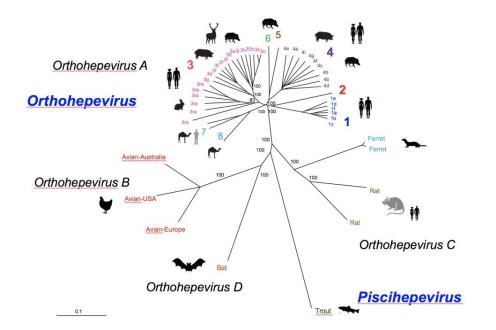
\includegraphics[width=0.5\linewidth]{imagenes/arbolfilogenetico.png}
	\caption[loftitle]{Esquema del árbol filogenético del virus de la hepatitis E, indicando sus principales reservorios \cite{Larrue2020}.} 
	\label{larrueimagen}
\end{figure}
\\\\Se hace una distinción epidemiológica entre los países en desarrollo y desarrollados. En los primeros, la transmisión del virus suele ser por una fuente de agua contaminada, debido a catástrofes naturales o pobres condiciones de saneamiento. En este caso, los afectados suelen ser jóvenes (15-30 años) y se ha comprobado la posibilidad de transmisión vertical, aumentando la mortalidad por el virus en mujeres embarazadas al 25\%. La mortalidad también es elevada (70\%) en pacientes con infección crónica del hígado concomitante.\\\\ Por otro lado, en los países desarrollados la transmisión suele ser principalmente zoonótica, por la ingestión de carne de cerdo contaminada mal cocinada. En estos genotipos se ha identificado un modo de transmisión potencial: la parenteral en pacientes inmunocomprometidos. Asimismo, la infección aguda afecta a personas de mayor edad (media de 55) y no se ha documentado transmisión vertical en este caso. Se destaca que la infección suele ser {\bf asintomática y autolimitante}, y que, en caso de presentar síntomas, estos son comunes e indiferenciables con las otras hepatitis virales (astenia, diarrea, naúseas, fiebre, ictericia...). En estos genotipos también se han descrito otros síntomas no asociados exclusivamente con el hígado. Aunque el mecanismo de causalidad aún no está claro, se sabe que el ciclo viral puede completarse en otros tejidos no hepáticos. Por tanto, pueden aparecer síntomas neurógicos en algunos pacientes (neuralgia amiotrófica, el síndrome de Guillain-Barré, meningoradiculatis). En contraposición con el pensamiento clásico de que el VHE solo puede desarrollarse con un cuadro agudo, se ha comprobado que, con el genotipo 3 y 4 del virus, ha habido casos de evolución crónica en pacientes inmunocomprometidos, que, sin tratamiento, pueden progresar rápidamente a cirrosis. Estos pacientes pueden ser: 
\begin{enumerate} 
\item Pacientes sometidos a quimioterapia
\item Pacientes infectados con el virus de la inmunodeficiencia humana (VIH) 
\item Pacientes con terapia inmunosupresiva ya sea por: 
\begin{enumerate}
	\item Recepción de trasplantes de órganos sólidos.
	\item Tratamiento a otras enfermedades (por ejemplo reumatismo inflamatorio).
\end{enumerate}
\end{enumerate}
En cuanto al diagnóstico, se diferencia entre el directo e indirecto. El primero se basa en la detección del ARN del virus en suero o heces por amplificación de la región del genoma conservada en ORF3/ORF2. El segundo se basa en la detección de los anticuerpos IgM (infección temprana) e IgG (protección inmunológica) contra el virus en sangre. Existen varios kits comerciales para realizar la medida con una gran sensibilidad. Sin embargo, se recomiendan únicamente en pacientes inmunocompetentes.\\\\
Por último, el tratamiento estándar es ribavirina, que es requerido únicamente en pacientes inmunocomprometidos que tienen riesgo de desarrollar un cuadro crónico de la infección. La prevención en países en desarrollo se basa en mejorar las condiciones de saneamiento. En el mundo desarrollado, en cambio, se recomienda el consumo de carne (esencialmente de cerdo) no cruda y bien cocinada, mientras que es un debate abierto la necesidad de cribado del virus en sangre antes de una transfusión. El cribado ya se realiza de manera rutinaria en Irlanda, Inglaterra, Países Bajos y Suiza. Se ha producido, además, una vacuna licenciada únicamente en China (Hecolin®, {\em (Xiamen Innovax Biotech)}), no integrada en programas de vacunación mundiales por la OMS debido a que no se ha probado su eficacia en pacientes inmunocomprometidos, en mujeres embarazadas ni en pacientes con una enfermedad hepática crónica. 
	
\subsubsection{Conclusiones}
Los autores reconocen abiertamente que la infección por hepatitis E es la causa principal de hepatitis aguda en el mundo. Por tanto, se deben realizar pruebas para la detección del virus no sólo a los pacientes con una hepatitis aguda sintomática, sino también a pacientes con síntomas neurológicos asociados con la hepatitis E (por el síndrome de Guillain-Barré por ejemplo). Para el diagnóstico basta con una prueba serológica para pacientes inmunocompetentes, pero para individuos inmunocomprometidos es necesario realizar otras técnicas moleculares que no requieran la detección de anticuerpos. Por último, también destacan la necesidad de tratar a pacientes con peligro de desarrollar una hepatitis crónica, y, por lo tanto, cirrosis, con ribavirina.

\subsection{Screening, diagnosis and risks associated with Hepatitis E virus infection}
Este artículo, redactado por Lhomme et al en mayo de 2019, recoge más información sobre las diferentes técnicas y ensayos para el diagnóstico del virus y sus manifestaciones clínicas \cite{Lhomme2019}.
\subsubsection{Resumen}
El conocimiento sobre el virus de ARNss de polaridad positiva de la hepatitis E ha ido aumentado significativamente en los últimos años. Se ha mejorado sustancialmente la realización de los ensayos serológicos y moleculares para la detección del virus. Asimismo, la disponibilidad de una medida estándar de la OMS ha permitido la comparación de los diferentes ensayos y la mejora de datos epidemiológicos del virus. Además, se recomienda además el cribado del ARN del virus en sangre para evitar la transmisión en individuos inmunocomprometidos. Se debe tener en cuenta estos métodos de diagnóstico cuando se sospecha de un paciente tiene un cuadro clínico de hepatitis. Hay que tener en cuenta que también se pueden presentar manifestaciones clínicas extrahepáticas. 
\subsubsection{Cuerpo del artículo}
Al principio del artículo se hace una introducción donde se dan los datos epidemiológicos según la OMS y el hecho de que el virus ha tomado importancia debido al descubrimiento de los genotipos que tienen impacto en los países desarrollados.\\\\
A continuación, se expone la taxonomía, destacando, igual que en el artículo anterior, que la especie {\em Orthohepevirus A} es el que suscita interés por la infección a mamíferos y, entre ellos, a humanos. Se hablan de los 4 genotipos importantes y brevemente de los otros 4. \\\\
{\bf Se ha documentado un caso de infección crónica en un paciente inmunocomprometido con el genotipo 7 del virus, que afecta a dromedarios. También se destaca que se han dado dos casos de infección con la especie {\em Orthohepevirus C}.}\\\\
Se describe detalladamente las características propias del virus, indicando qué dominios existen dentro de los ORFs del virus y la función de cada uno de ellos. Esto se puede visualizar en la figura \ref{lhommegenoma}.\\\\
\begin{figure} [h!] 
	\centering
	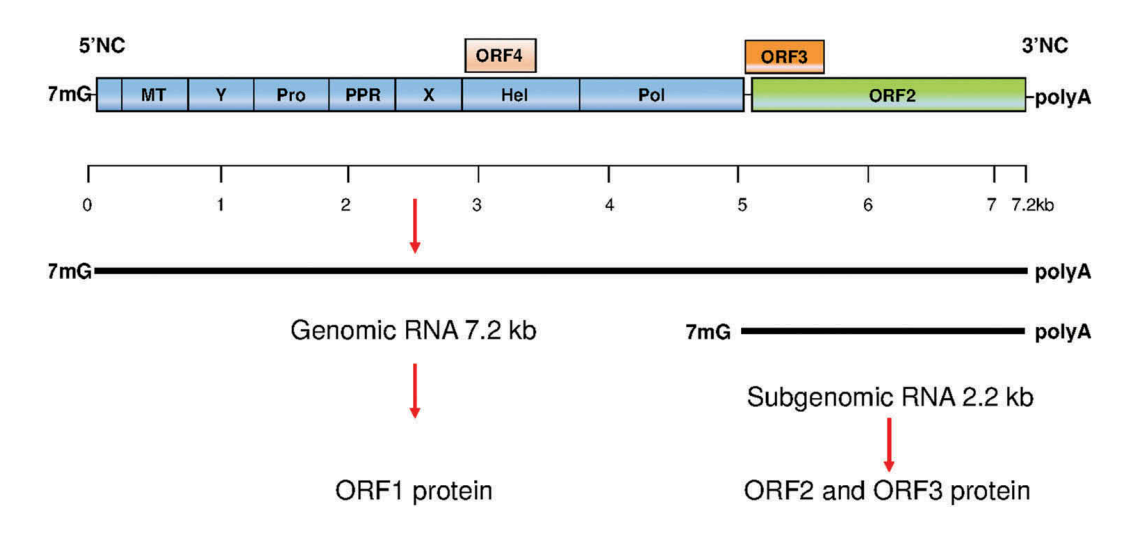
\includegraphics[width=0.75\linewidth]{imagenes/genoma VHE.png}
	\caption[loftitle]{Esquema de la organización del genoma del VHE. Tomado de Lhomme et al (2019) \cite{Lhomme2019}}
	\label{lhommegenoma}
\end{figure}
\\\\Por otro lado, antes de meterse de lleno con los métodos de diagnóstico, incluye una gráfica que muestra la evolución de los diferentes marcadores que ayudan al diagnóstico de la hepatitis E (Figura \ref{lhommemarcador}). Entre ellos, se indica la evolución del marcador bioquímico que mide la actividad del hígado: Alanina aminotransferasa o ALT. También se indica que el ARN y los antígenos del virus se encuentran en heces y sangre durante las primeras semanas de infección. Por su parte, se marca la aparición de la respuesta inmunitaria; primero se da la respuesta IgM, que indica infección temprana y, poco después, la IgG, que es la que permanece y persiste por varios años (inmunización).
\begin{figure} [h!] 
	\centering
	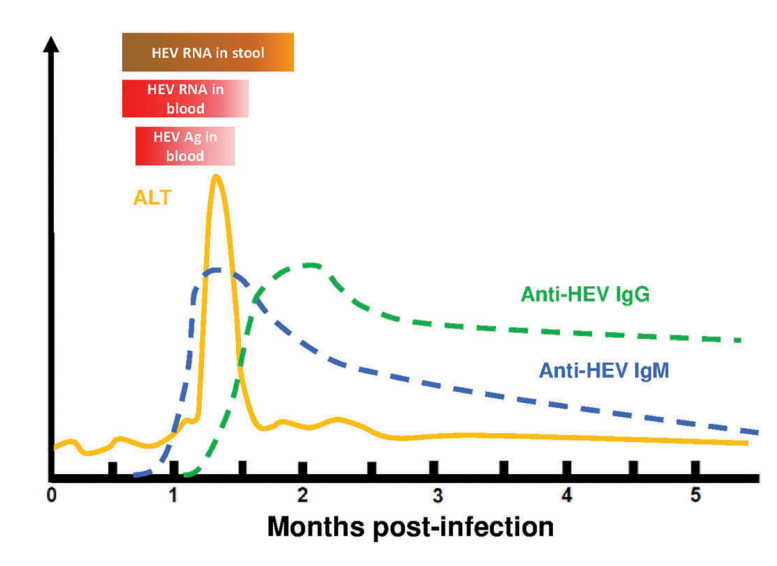
\includegraphics[width=0.75\linewidth]{imagenes/marcadoresHEV.png}
	\caption[loftitle]{Evolución de los marcadores por infección de VHE. Tomado de Lhomme et al (2019) \cite{Lhomme2019}}
	\label{lhommemarcador}
\end{figure}
\\\\En cuanto a las técnicas de diagnóstico, se va a resumir los tipos, las ventajas e inconvenientes de cada una en la tabla \ref{tabladiagn}. 
\begin{table}[h!]
	\begin{tabular}[c]{||c|c|c|c|c||}
		\hline
		{\bf Ensayo} & {\bf Método} & {\bf Uso} & {\bf Comentario} & {\bf Kit comercial} \\
		\hline
		{\bf IgM anti-VHE} & \parbox[c]{3.5 cm}{ELISA Inmunocromatografía} & Infección aguda & \multirow{2}{*}{\parbox[c]{3 cm}{Diferentes formas de llevarlas a cabo. Uso limitado en inmunocomprometidos. Reactividad cruzada}} & \parbox[c]{2.25 cm}{Wantai- HEV ELISA IgM. Wantai HEV IgM Rapid test} \\
		\cline{1-1}\cline{2-2}\cline{3-3}\cline{5-5}
		{\bf IgG anti-VHE} & \parbox[c]{3.5 cm}{ELISA Inmunocromatografía} & \parbox[c]{3 cm}{Seroprevalencia. Protección natural. Eficiencia vacuna. Posibilidad de reinfección} & & \parbox[c]{2 cm}{Wantai HEV ELISA IgG} \\
		\hline
		{\bf ARN VHE} & \parbox[c]{3 cm}{Medida ácidos nucleicos. RT-PCR. LAMP} & \parbox[c]{3 cm}{Infección aguda. Confirmar cronicidad. Respuestas antivirales. Cribado del donante} & \parbox[c]{3.5 cm}{Poca duración de la viremia. Necesaria estandarización del método. Ventaja en desórdenes inmunológicos}  & \parbox[c]{2 cm}{Altona Diagnostics Real Star HEV RT-PCR v2.0} \\
		\hline
		{\bf Antígeno VHE} & \parbox[c]{3.75 cm}{Enzimoinmunoensayo} & \parbox[c]{3 cm}{Infección aguda. Ags permanecen más tiempo en infección crónica} & \parbox[c]{2.5 cm}{82\% de concordancia con ARN VHE}  & \parbox[c]{2 cm}{Wantai ELISA sándwich} \\
		\hline	
	\end{tabular}
\caption{Resumen de las características más importantes de cada método de diagnóstico}
\label{tabladiagn}
\end{table}
\\\\Se defiende, también, la estrategia de diagnóstico publicado por la Asociación Europea del Estudio del Hígado (EASL), que recomienda una combinación de las técnicas serológicas y de las moleculares, teniendo en cuenta que {\bf en los pacientes con inmunosupresión no se van a detectar ni IgM ni IgG.}\\\\
Para finalizar el artículo, los autores comentan los riesgos asociados con la infección del VHE, indicando, como en el artículo anterior, que es una infección asintomática y autolimitante. Los pacientes sintomáticos, presentan manifestaciones clínicas comunes a las demás hepatitis. Sin embargo, en este artículo se resalta que {\bf las manifestaciones extrahepáticas no son solo neurológicas, sino que también existen manifestaciones renales, hematológicas, e, incluso, la hepatitis E puede estar ligada con pancreatitis.}
\subsubsection{Conclusiones}
\begin{itemize}
	\item El interés de la hepatitis E se ha incrementado en los últimos 20 años tras el descubrimiento de los reservorios animales y la caracterización de una posible hepatitis crónica en pacientes inmunocomprometidos.
	\item La mejora de técnicas serológicas ha permitido un estudio de seroprevalencia. Sin embargo, es difícil comparar los resultados debido a la falta de estandarización entre los ensayos.
	\item No hay una estrategia común para el diagnóstico de la hepatitis E. La Asociación Europea del estudio del hígado (EASL) recomienda la detección de anticuerpos y el ARN del virus. Se necesitan más estudios para confirmar la utilidad de la medida de los antígenos del virus en el diagnóstico.
	\item Al ser una infección asintomática, algunos donantes de sangre pueden portar el virus sin saberlo. En algunos países ya se realizan cribados sanguíneos del VHE. 
	\item Los síntomas de la hepatitis E son indistinguibles a otras hepatitis virales. Es necesario, por tanto, que también se tenga en cuenta la hepatitis E a la hora de buscar un diagnóstico, sobre todo cuando este paciente presenta manifestaciones extrahepáticas. 
	\item Se deben desarrollar otros medicamentos eficaces o realizar nuevos ensayos clínicos para el tratamiento para suplir los casos en que la ribavirina no sea eficaz.
	\item Por último, es necesario desarrollar una estrategia óptima de prevención. La eficacia vacuna existente en China no está probada en el colectivo de riesgo. Además, se están encontrando otros reservorios animales y otros genotipos que pueden infectar a humanos.
\end{itemize}

\subsection{Hepatitis E virus infection}
Este artículo de Nature es más antiguo, de 2017, pero es de gran interés ya que trata de manera detallada todos los aspectos relacionados con el virus tanto en el mundo desarrollado como en países en desarrollo \cite{Kamar2017}. Además, la revista de publicación tiene un excelente índice de impacto.
\subsubsection{Resumen}
El VHE es la causa principal de hepatitis aguda en todo el mundo. Últimamente, el interés de este virus esta creciendo al ser reconocido como endémico en algunos países desarrollados. La transmisión es principalmente zoonótica y se han documentado casos de transmisión parenteral a pacientes inmunocomprometidos. El diagnóstico puede realizarse a través de la medida de anticuerpos anti-VHE, del propio ARN o de antígenos de la cápsida viral en sangre y/o heces. Existe únicamente una vacuna licenciada en China. En individuos inmunocompetentes la infección suele ser autolimitante, mientras que en individuos inmunocomprometidos el tratamiento suele basarse en una disminución de dosis de medicamentos inmunosupresivos incluyendo o no el antiviral ribavirina. 
\subsubsection{Cuerpo del artículo}
Además de tocar los temas ya tratados en los artículos anteriores, este artículo se destaca por la descripción detallada de la epidemiología y transmisión de los diferentes genotipos en las diferentes zonas, tal y como se muestra en la figura \ref{kamarmapa}.\\\\
\begin{figure} [h!] 
	\centering
	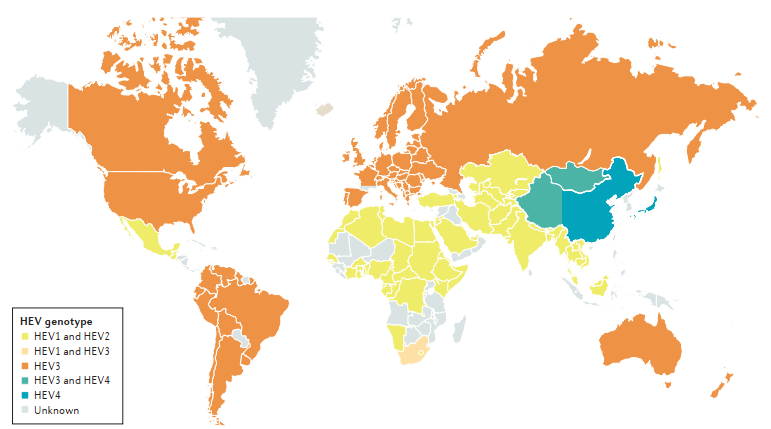
\includegraphics[width=0.80\linewidth]{imagenes/mapaepidemiologia.png}
	\caption[loftitle]{Presencia de los diferentes genotipos en el mundo \cite{Kamar2017}.}
	\label{kamarmapa}
\end{figure}
Asimismo, describe el ciclo de vida del virus en el hepatocito, indicando que hay muchos procesos moleculares que aún no se conocen. Como ejemplo, no se conoce la molécula que actúa como receptor del virus. Además, se cree que en el ciclo de vida del virus cuasienvuelto y el virus desnudo actúan diferentes moléculas. El ciclo que más se conoce es el del virus envuelto y se representa en la figura \ref{kamarciclo}.
\begin{figure} [h!] 
	\centering
	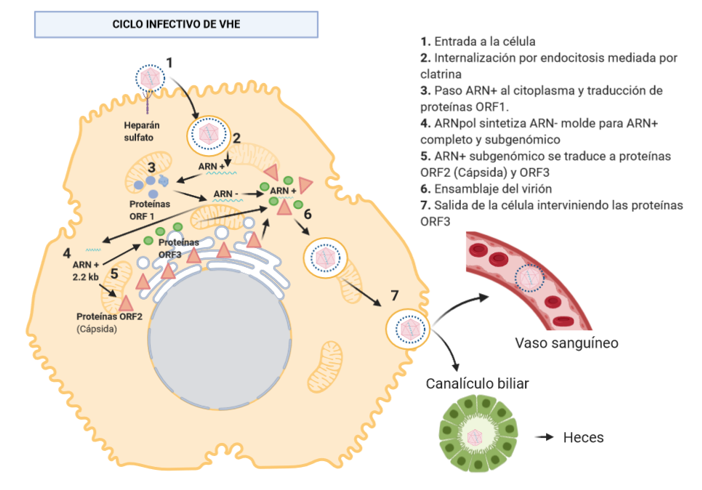
\includegraphics[width=0.80\linewidth]{imagenes/cicloinfectivo.png}
	\caption[loftitle]{Descripción del ciclo infectivo. Imagen propia adaptada de  \cite{Kamar2017}.}
	\label{kamarciclo}
\end{figure}
\\\\Por último, también incluye una estrategia de tratamiento dependiendo si la infección se produce en individuos inmunocompetentes (que no suelen precisar tratamiento) e inmunocomprometidos, parándose en cada caso (Figura \ref{kamartrata}). Se recalca además la importancia de buscar nuevos antivirales que sustituyan a la ribavirina en caso de que no haya respuesta por parte del paciente.
\begin{figure} [h!] 
	\centering
	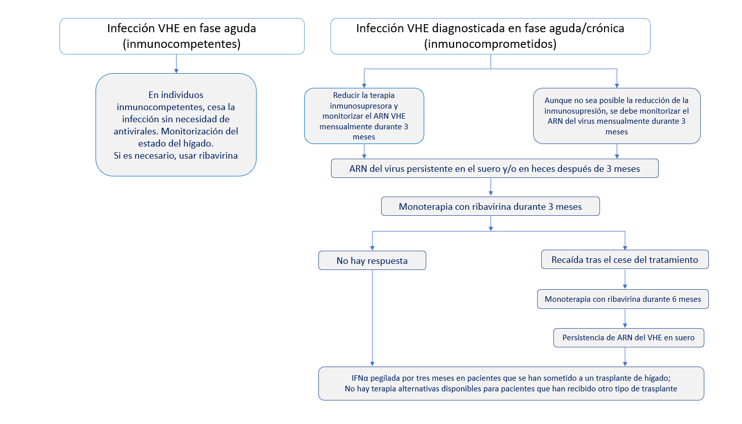
\includegraphics[width=\linewidth]{imagenes/tratamiento.png}
	\caption[loftitle]{Estrategia de tratamiento. Imagen propia adaptada de  \cite{Kamar2017}.}
	\label{kamartrata}
\end{figure}
\subsubsection{Conclusiones} 
\begin{itemize}
\item Para la prevención, además del debate sobre el cribado, la OMS dispone de una guía para evitar la transmisión del virus por fuente de agua contaminada. En los países desarrollados es necesario realizar cambios en la ganadería e integrar buenas prácticas en la cocina para evitar alimentos contaminados.
\item Hay mucho desconocimiento acerca de los mecanismos moleculares que integran el ciclo de vida del virus. Es necesario seguir estudiándolo con el objetivo de poder realizar diagnóstico y/o terapias más efectivas.
\item No hay vacunas alternativas a la existente en China en desarrollo.
\item No hay tratamiento eficaz que pueda sustituir a la ribavirina en caso de que sea poco eficaz. No obstante, existen ensayos que muestra que los inhibidores de cacineurina ayudan a la eliminación del virus. Asímismo, se está probando también la eficacia de otros compuestos como el sofosbuvir.
\item No hay que subestimar al VHE, pues está demostrando ser uno de los virus zoonóticos que más éxito tienen a la hora de afectar a los humanos. 
\end{itemize}

\section{Conclusiones finales}
Tras la búsqueda de los artículos más relevantes y actualizados de la patología de la Hepatitis E, se puede destacar los siguientes puntos:
\begin{itemize}
	\item 
	La infección por VHE ha dejado de considerarse anecdótica y asociada a viajero en países desarrollados, siendo los genotipos 3 y 4 los más frecuentes en estos países. La transmisión de estos genotipos es zoonótica, siendo el ganado porcino el principal reservorio. 
	\item 
	Los genotipos 3 y 4 pueden producir hepatitis crónica en personas inmunocomprometidas, principalmente trasplantados.
	\item 
	Existe relación de infección por genotipos 3 y 4 y manifestaciones extrahepáticas (neurológicas, renales y hematológicas), aunque la relación causa efecto aún está en estudio.
	\item 
	Existe controversia respecto a la necesidad de cribado del VHE en donantes de sangre y órganos.
	\item 
	Falta por establecer dosis y tiempo del tratamiento con ribavirina
	\item 
	Existen muchos ensayos para diagnóstico serológicos, aunque ninguno ha sido aún aprobado por la FDA. Falta estandarización en estos ensayos
	\item 
	En cuanto a la prevención, se basa en medidas higiénico sanitarias en países en vías de desarrollo y evitar consumo de carnes poco cocinadas. Solo existe una vacuna licenciada en China, denominada Hecolin® {\em (Xiamen Innovax Biotech)}. La OMS no la ha integrado en programas de vacunación globales porque se necesita probar su eficacia con respecto a otros genotipos y su seguridad en pacientes de riesgo.
\end{itemize}
Por consiguiente, es necesario continuar los esfuerzos de investigación en los puntos destacados donde hay desconocimiento. Al final, el objetivo es poder realizar un buen tratamiento y, sobre todo, crear una vacuna global para lograr una prevención eficaz.

\section{Anexo: Fórmulas}
Con el objetivo de practicar la implementación de fórmulas en LaTeX, se ha creado esta sección aparte, ya que el tema tratado no implica el trabajo con fórmulas matemáticas.\\\\


\bibliography{biblio_proyectofinal}
\bibliographystyle{unsrt}		
\end{document}